\documentclass[12pt]{extarticle}
%Some packages I commonly use.
\usepackage[portuguese]{babel}
\usepackage{graphicx}
\usepackage{framed}
\usepackage[normalem]{ulem}
\usepackage{amsmath}
\usepackage{amsthm}
\usepackage{amssymb}
\usepackage{amsfonts}
\usepackage{enumerate}
\usepackage[utf8]{inputenc}
\usepackage{float}
\usepackage{gensymb}
\usepackage[top=1 in,bottom=1in, left=1 in, right=1 in]{geometry}
\usepackage{multirow}
\usepackage{caption}
\usepackage{subcaption}
\usepackage[utf8]{inputenc}

%A bunch of definitions that make my life easier
\newcommand{\matlab}{{\sc Matlab} }
\newcommand{\cvec}[1]{{\mathbf #1}}
\newcommand{\rvec}[1]{\vec{\mathbf #1}}
\newcommand{\ihat}{\hat{\textbf{\i}}}
\newcommand{\jhat}{\hat{\textbf{\j}}}
\newcommand{\khat}{\hat{\textbf{k}}}
\newcommand{\minor}{{\rm minor}}
\newcommand{\trace}{{\rm trace}}
\newcommand{\spn}{{\rm Span}}
\newcommand{\rem}{{\rm rem}}
\newcommand{\ran}{{\rm range}}
\newcommand{\range}{{\rm range}}
\newcommand{\mdiv}{{\rm div}}
\newcommand{\proj}{{\rm proj}}
\newcommand{\R}{\mathbb{R}}
\newcommand{\N}{\mathbb{N}}
\newcommand{\Q}{\mathbb{Q}}
\newcommand{\Z}{\mathbb{Z}}
\newcommand{\<}{\langle}
\renewcommand{\>}{\rangle}
\renewcommand{\emptyset}{\varnothing}
\newcommand{\attn}[1]{\textbf{#1}}
\theoremstyle{definition}
\newtheorem{theorem}{Theorem}
\newtheorem{corollary}{Corollary}
\newtheorem*{definition}{Definition}
\newtheorem*{example}{Example}
\newtheorem*{note}{Note}
\newtheorem{exercise}{Exercise}
\newcommand{\bproof}{\bigskip {\bf Proof. }}
\newcommand{\eproof}{\hfill\qedsymbol}
\newcommand{\Disp}{\displaystyle}
\newcommand{\qe}{\hfill\(\bigtriangledown\)}
\setlength{\columnseprule}{1 pt}
\usepackage[utf8]{inputenc}

\title{Aulas 9 e 10 - Campo Elétrico ($\vec{E}$)}
\author{Felipe Salvador}
\date{Atualizado em \today}

\begin{document}

\maketitle

\section{Introdução - A intuição por trás do conceito}

Na aula passada, vimos o que era a Lei de Coulomb, a lei que expressa a força de 2 cargas elétricas (pontuais):
\begin{equation}
    F = \frac{K_0\,|q_1|\,|q_2|}{d^2}
\end{equation}
\noindent em que $K_0$ era uma constante eletrostática, os $q_1,\,q_2$ são os valores das cargas elétricas envolvidas e $d$ é a distância entre elas.

No entanto, essa Lei depende que 2 cargas estejam no espaço para que a gente possa saber a força exercida, além da direção da força. Isso não é ideal, uma vez que a maioria das vezes eu só tenho 1 carga elétrica no espaço. Então, as perguntas a serem respondidas são: \textbf{Será que é possível ter uma ideia da direção e do módulo da força sem precisar colocar a 2ª carga no espaço? Será possível construir uma ideia de como a força é no espaço inteiro para que, quando eu coloque a 2ª carga, basta arrumar só o módulo da força?}

A resposta é sim. Os benefícios de conseguir fazer isso são esses:
\begin{itemize}
    \item Consigo mapear como seria a força no espaço inteiro que estou trabalhando, sem precisar colocar a segunda carga.
    \item Me dá uma ideia do comportamento (análise qualitativa) de como a força se comporta quando coloco a 2ª carga em diferentes lugares;
    \item Consigo extrair as informações importantes da força elétrica (direção e a escala do módulo) sem precisar colocar a 2ª carga.
\end{itemize}

Isso é fantástico, sem precisar ter uma 2ª carga no problema, eu consigo fazer analisar e estudar o comportamento geral da 1ª, sem qualquer perda de informação e prever o comportamento da força elétrica. As únicas 2 informações, que dependem da 2ª carga e restariam determinar para a força, seriam o sentido da força (que depende do sinal da 2ª carga) e o módulo da força (valor nominal da 2ª carga). 

Por isso, criou-se o conceito de \textbf{Campo Elétrico}, que é \textbf{uma quantidade que depende somente da 1ª carga e consegue me dizer sobre o comportamento geral da força elétrica no espaço, sem precisar colocar a 2ª carga.}

Ele carrega as informações mais importante quando estudamos as forças elétricas, porque ele traz as informações da direção e a escala do módulo da força no espaço inteiro (sem ser só num ponto, como na Lei de Coulomb).

\section{Fórmula do Campo Elétrico}
Para encontrar o valor Campo Elétrico, pegamos a Lei de Coulomb e separamos as cargas:
\begin{equation}
    F = \frac{K_0\,|q_1|}{d^2}\,|q_2|
\end{equation}

\textbf{O que está na fração é definido como o campo elétrico de uma carga pontual:}
\begin{equation}
    \boxed{E = \frac{K_0\, |q_1|}{d^2}}
\end{equation}
\noindent lembrando que para 2 dimensões, a distância $d$ é dada como:
\begin{equation}
    d = \sqrt{(x-x_0)^2 + (y-y_0)^2}
\end{equation}
\noindent em que $(x_0,y_0)$ é a posição da carga $q_1$ e $(x,y)$ é um ponto qualquer no espaço que a carga está.

Com isso, podemos reescrever a Lei de Coulomb como:
\begin{equation} \label{eq:force_field}
    F = E\,|q_2| \implies \boxed{F= qE}
\end{equation}
\noindent na linguagem de vetores (expressa por flechas), a equação é reescrita como:
\begin{equation}
    \vec{F} = q\vec{E}
\end{equation}

Como a força é dada em Newton e a carga é dada em Coulomb, a unidade do campo elétrico é:
\begin{equation}
    [F]=[q][E] \implies[E]=\frac{[F]}{[q]} \implies [E]= \frac{N}{C}
\end{equation}

Outra unidade usada para o campo elétrico (que veremos de onde vem, na próxima aula) é a seguinte:
\begin{equation}
    [E]= \frac{V}{m}
\end{equation}

As duas unidades dadas acima são equivalentes. Sobre o sentido do campo elétrico, ele respeitar a seguinte convenção:
\begin{itemize}
    \item Caso a carga que esteja gerando o campo seja uma carga positiva, o campo estará apontando para fora da carga
    \item Caso a carga que esteja gerando o campo seja negativa, o campo estará apontando para a carga.
\end{itemize}

\begin{figure}[H]
     \centering
     \begin{subfigure}[b]{0.45\textwidth}
         \centering
         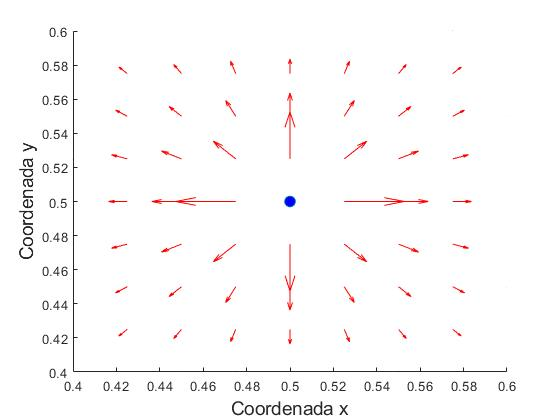
\includegraphics[width=\textwidth]{simu_campo_eletrico_carga_+.jpg}
         \caption{Simulação de um campo elétrico gerado por uma carga pontual positiva no ponto (x,y) = (0.5, 0.5)}
         \label{fig:field_+}
     \end{subfigure}
     \quad\quad
     \begin{subfigure}[b]{0.45\textwidth}
         \centering
         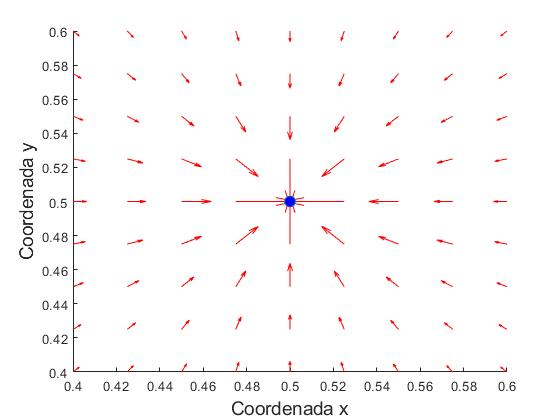
\includegraphics[width=\textwidth]{simu_campo_eletrico_carga_-.jpg}
         \caption{Simulação de um campo elétrico gerado por uma carga pontual negativa no ponto (x,y) = (0.5, 0.5)}
         \label{fig:field_-}
     \end{subfigure}
        \caption{Simulação dos campos elétricos gerados por uma carga positiva (imagem à esquerda) e uma carga negativa (imagem à direita)}
        \label{fig:electric_field}
\end{figure}

Uma questão interessante, é quando temos problemas com diversas cargas no espaço e queremos saber para onde iria uma carga pequena (que damos o nome de \textbf{carga de prova}). Para isso, vamos usar um exemplo para estudar:

\begin{figure}[H]
    \centering
    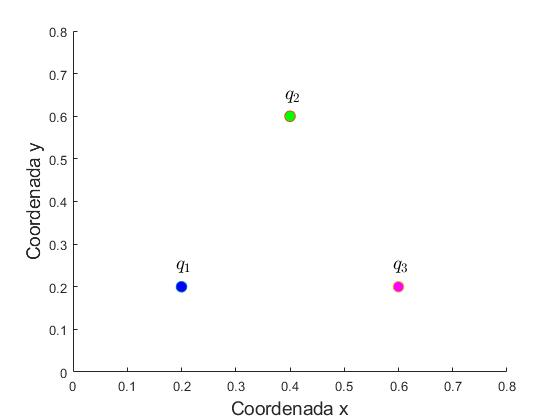
\includegraphics[width=0.6\textwidth]{ex_1.jpg}
    \caption{3 Cargas no espaço}
    \label{fig:ex_1}
\end{figure}

Vimos na aula passada que quando múltiplas cargas aplicam uma força elétrica sobre, nesse exemplo $q_2$, a força que $q_2$ sofrem é:
\begin{equation}
    F_2 = F_{12} + F_{32}
\end{equation}
\noindent $F_{12}$ é a força que a carga 1 ($q_1$) aplica na carga 2 ($q_2$) e a mesma coisa para $F_{32}$: a força que a carga 3 aplica em 2. Se substituir a fórmula da força em termos do campo elétrico:
\begin{align*}
    &F_{12} = E_1\,q_2\\
    &F_{23} = E_3\,q_2
    \implies F_2 = E_1\,q_2 + E_3\,q_2\\
\end{align*}
Então:
\begin{equation}
    F_2 = q_2\left(E_1 + E_3 \right) = E\,q_2 \implies E = E_1 + E_3
\end{equation}

Na forma vetorial: 
\begin{equation}
    \vec{E} = \vec{E}_1 + \vec{E_3}
\end{equation}

Isso me diz que: \textbf{Num espaço com várias cargas, a força que uma carga sofre é o produto da soma dos campos elétricos das outras cargas envolvidas com o valor da carga.}

Para visualizar, vamos analisar como seria o campo elétrico gerado pelas cargas 1 e 3 ($q_1\,e\,q_3$):
\begin{figure}[H]
    \centering
    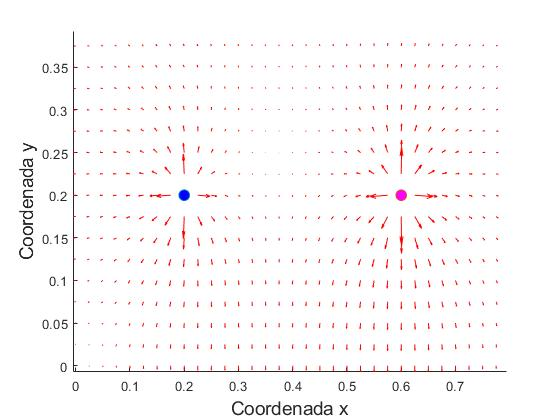
\includegraphics[width=0.6\textwidth]{multi_charge_system.jpg}
    \caption{Campo elétrico formado por 2 cargas elétricas $q_1$ e $q_3$, quando ambas são positivas. As posições das cargas são: $q_1=(0.2,\,0.2)$ e $q_3=(0.2,\,0.6)$}
    \label{fig:multi_system}
\end{figure}

Um caso interessante é quando analisar é quando uma carga é positiva e a outra é negativa. Para essa configuração, damos o nome de \textbf{dipolo} (di + polo - 2 pólos):
\begin{figure}[H]
     \centering
     \begin{subfigure}[b]{0.45\textwidth}
         \centering
         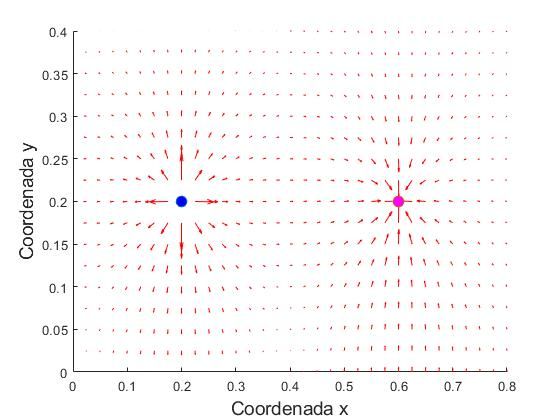
\includegraphics[width=\textwidth]{dipole.jpg}
         \caption{Simulação de um campo elétrico gerado por 2 cargas pontuais: uma positiva no ponto (x,y) = (0.2, 0.2) e uma negativa no ponto (x,y) = (0.6, 0.2)}
         \label{fig:dipole_field}
     \end{subfigure}
     \quad\quad
     \begin{subfigure}[b]{0.45\textwidth}
         \centering
         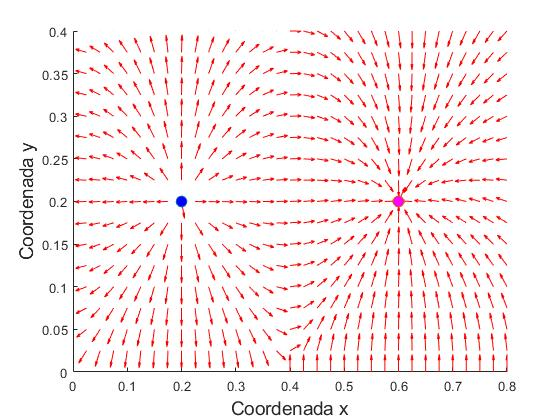
\includegraphics[width=\textwidth]{dipole_2.jpg}
         \caption{(Desconsiderando o módulo) Simulação de um campo elétrico gerado por 2 cargas pontuais: uma positiva no ponto (x,y) = (0.2, 0.2) e uma negativa no ponto (x,y) = (0.6, 0.2)}
         \label{fig:field_-}
     \end{subfigure}
        \caption{Diagrama do campo elétrico gerado por um par de cargas: 1 positiva e 1 negativa.}
        \label{fig:dipole_field_no_size}
\end{figure}

\section{Campo Elétrico Uniforme}

Uma das configurações mais importantes de Campo Elétrico é quando ele aponta para uma direção e sentido definidos e o seu módulo é constante em todo espaço. Nesse caso, é o que chamamos de \textbf{Campo Elétrico Uniforme}, em que é uma das configurações mais simples e úteis de se fazer/analisar.

A forma mais simples de construir um campo elétrico uniforme é quando colocamos 2 placas, uma com cargas positivas e a outra com cargas negativas. Essa configuração é chamada de \textbf{capacitor}:
\begin{figure}[H]
    \centering
    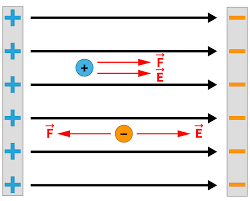
\includegraphics[width=0.5\textwidth]{campo_eletrico_uniforme.png}
    \caption{Diagrama do campo elétrico de um capacitor}
    \label{fig:uniform_electric}
\end{figure}

\textbf{Perceba na figura, quando a carga colocada é positiva, a força e o campo elétrico possuem o mesmo sentido, enquanto se ela for negativa, os sentidos são opostos.}

Com esse campo, nós podemos fazer uma previsão da aceleração, velocidade e posição de uma carga num campo elétrico uniforme. Pela equação (\ref{eq:force_field}):
\begin{equation}
    F=q\,E
\end{equation}

Pela Segunda Lei de Newton, sabemos que a força é: $F =ma$, logo:
\begin{equation}
    m\,a=q\,E \implies \boxed{a = \frac{q\,E}{m}}
\end{equation}

Lembrando que essa aceleração é na direção do campo elétrico uniforme, ou seja, se o campo elétrico for na direção horizontal, a aceleração também será na vertical. Para encontrar a velocidade, precisa-se usar as equações da cinemática.

\section{Campo Elétrico dentro de um condutor oco e fechado}

Vimos na aula de introdução à eletricidade, que quando aproximamos uma carga elétrica a um condutor, esse condutor vai ser induzido, conforme a figura abaixo:
\begin{figure}[H]
    \centering
    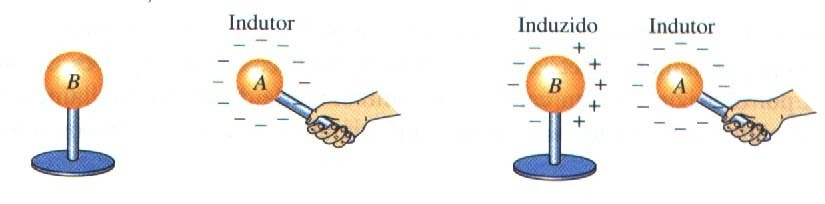
\includegraphics[width=0.8\textwidth]{eletrizacao_por_inducao.jpg}
    \caption{Um condutor sendo induzido eletricamente por uma esfera eletrizada}
    \label{fig:induction}
\end{figure}

Isso acontece por causa que a esfera eletrizada está gerando campo elétrico e, quando a esfera se aproxima do condutor, gera uma força sobre as cargas elétricas que estão no condutor (lembrando que tem uma mesma quantidade de cargas positivas e negativas). Com isso, como a esfera da figura é carregada negativamente, as cargas positivas do condutor são atraídas e as cargas negativas do condutor são repelidas. 

Uma questão importante, é que essas cargas induzidas, \textbf{estão na superfície do condutor, nunca dentro.}

Para entender melhor, vamos separar a questão em 2 casos:
\begin{itemize}
    \item Quando a esfera eletrizada está longe e o condutor não está submetido ao campo elétrico gerado pela esfera;
    \item Quando a esfera eletrizada está próxima do condutor e o condutor sofre a indução e, consequentemente, a ação do campo elétrico da esfera.
\end{itemize}

No primeiro caso, como não há campo elétrico gerado pela esfera na posição do condutor, logo dentro do condutor, o campo elétrico é 0.

Já no segundo caso, a esfera eletrizada gera o campo elétrico, que induz a eletrização das cargas do condutor. \textbf{Porém, verificou-se experimentalmente que a indução das cargas no condutor acontece de forma a cancelar o campo elétrico da esfera dentro do condutor.} É uma reação do próprio condutor a fim de manter a quantidade inicial (campo elétrico =0).

Esse fenômeno chama-se \textbf{Blindagem Eletrostática} e é usada para proteger/ resguardar equipamentos e pessoas de choques que possam ser induzidos por raios atmosféricos ou outras fontes.

Por isso, \textbf{um condutor fechado na presença de um campo elétrico externo, reage de forma que o campo elétrico dentro dele é sempre 0.}

\textbf{Também, no caso de um condutor com cargas, as cargas vão ficar na superfície, de forma que o campo elétrico dentro dele é sempre 0.}

\begin{figure}[H]
    \centering
    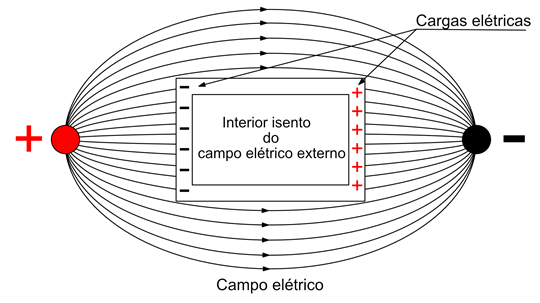
\includegraphics[width=0.5\textwidth]{campo-eletrico.png}
    \caption{Diagrama do que ocorre quando se tem um campo elétrico externo aplicado e um condutor fechado.}
    \label{fig:conductor}
\end{figure}


\end{document}
